\chapter{Implementation}
\label{chap3}
\label{sec:pipeline}
\section{Overview}
There are a number of steps that are required in order for the system to be able to return the desired output.
We must first gain an understanding of how the model works. At a very basic level the model works as follows:
\bigbreak
The model will aim to process a previously unseen sample (an invoice not in the training set), look through each piece of
text / word in every bounding box, determine the words relationship with other words via its position. Then based on the
annotated examples it has `learned from', determine which labels (if any) should apply to each word in the unseen
document. The words and their label should be returned by the model.\\
\#\#\ This section may not be needed dependent on the detail in the previous section. \#\#\

\section{Dataset Preparation}
\label{sec:dataset}
To fine-tune \#\#\ fine-tune needs to be explained in the context of transfer learning \#\# \\
the model on the custom invoice dataset, the dataset needs to be prepared. The dataset needs to be annotated
with labels. These labels are the labels the model will predict for fields on an invoice during inference.
\bigbreak
The annotation process is both extremely tedious and time-consuming but has to be done with great care and precision
for optimal results from the model. If the annotations in the training set are not accurate the model will never be able
to infer the correct labels. If there is too many mistakes in the training set then the model may fail to converge.
\bigbreak
Initial attempts at using PDF viewers and annotating the invoices with them proved extremely slow and problematic.
Most readers are simply not designed for the level of annotation that is required for model training. This was only
found out after testing numerous applications, including Master PDF Editor, Acrobat Reader and Zathura PDF. All in
all about eight such applications were tested before the change of course to specialised annotation software.
\bigbreak
There are some open-source annotation software that can be used to annotate documents for ML purposes. This process was
also very time-consuming. A lot of the software out there was difficult to install / had to be installed from
scratch. Having tried 5 or 6 different applications, including LabelMe~\autocite{wadaLabelmeImagePolygonal2022},
VGG Image Annotator\~autocite{duttaAnnotationSoftwareImages2019} and Label Studio~\autocite{LabelStudioOpen}, it
is clear that the vast majority are designed for image classification and not NLP. After reading countless articles
about how to use the tools, none of them allowed for the swift annotation of invoices. Some also have steep learning
curves. More often than not the applications had clunky UIs and would be extremely buggy. At this point a decision
was taken to try and find some student rates for professional annotation software.
\bigbreak
There are a number of professional annotation tools and having researched them thoroughly, Light-Tag~\autocite{LightTagTextAnnotation}
and UBIAI~\autocite{EasyUseText}, were the options attempted. Light-Tag proved extremely expensive. But UBIAI was the
most affordable option, and what an option. The software was incredibly straightforward to use and the support
team (the founder) was very helpful. I reached out to the support team for help with the software as I was
looking for a student discount. The founder, Walid, was the same person who had written a number of articles about
the use and training of the original LayoutLM model for invoice training~\autocite{EasyUseTexta}~\autocite{EasyUseTextb}
and~\autocite{amamouFineTuningLayoutLMV22022}, which were very helpful in the writing of the training script.\\
Talking with Walid, he was very interested in this project. Walid was doing something similar in the area of semi-structured
document understanding and was also frustrated by the annotation tools available. This is how UBIAI was born. With a very generous
student discount secured for the project and some great conversations about the structure of the model etc. the
next step was to use the software to get the annotation done.
\bigbreak
The steps are as follows:
\begin{enumerate}
	\item \textbf{Label Creation}: involves planning and creating the desired labels. The labels denote the key pieces of information
	      that are of interest. So the appropriate labels must be created for the relevant fields.\\
	      For this project these are the labels which are relevant for the desired output and functionality of this part of the system.
	      \begin{figure}[H]
		      \centering
		      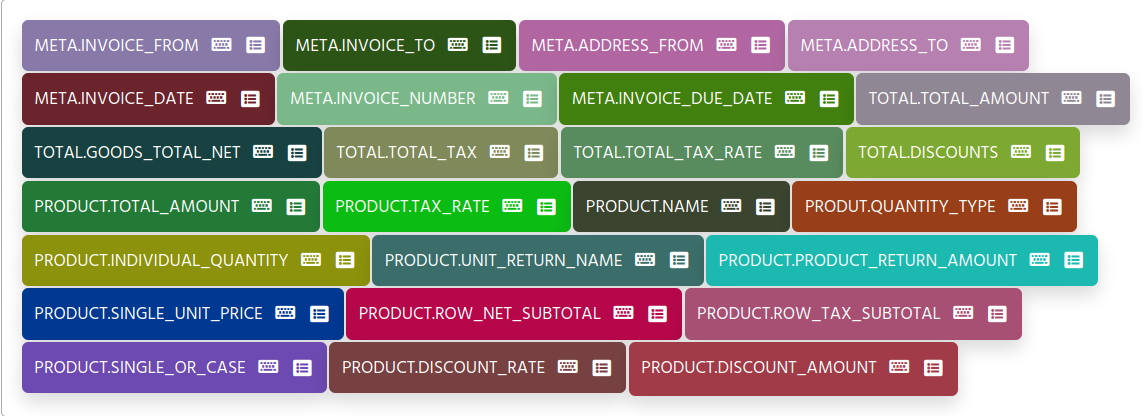
\includegraphics[width=0.9\textwidth]{figures/training_labels.png}
		      \caption{Training and Inference Labels created for the system}
		      \label{fig:training_labels}
	      \end{figure}
	\item \textbf{Annotation}: of all invoices in the dataset by applying the labels to the words. The annotation process is
	      very straightforward, the labels are color-coded and have customizable keyboard shortcuts. The text from the document
	      is OCR'd and displayed sequentially in the bottom half of the screen. The PDF document is displayed to the side.
	      One can simply highlight an area of text on the document and the current enabled label is applied to the text.
	      As text on the document is labeled the corresponding text is highlighted in the OCR'd output section.
	      \begin{figure}[H]
		      \centering
		      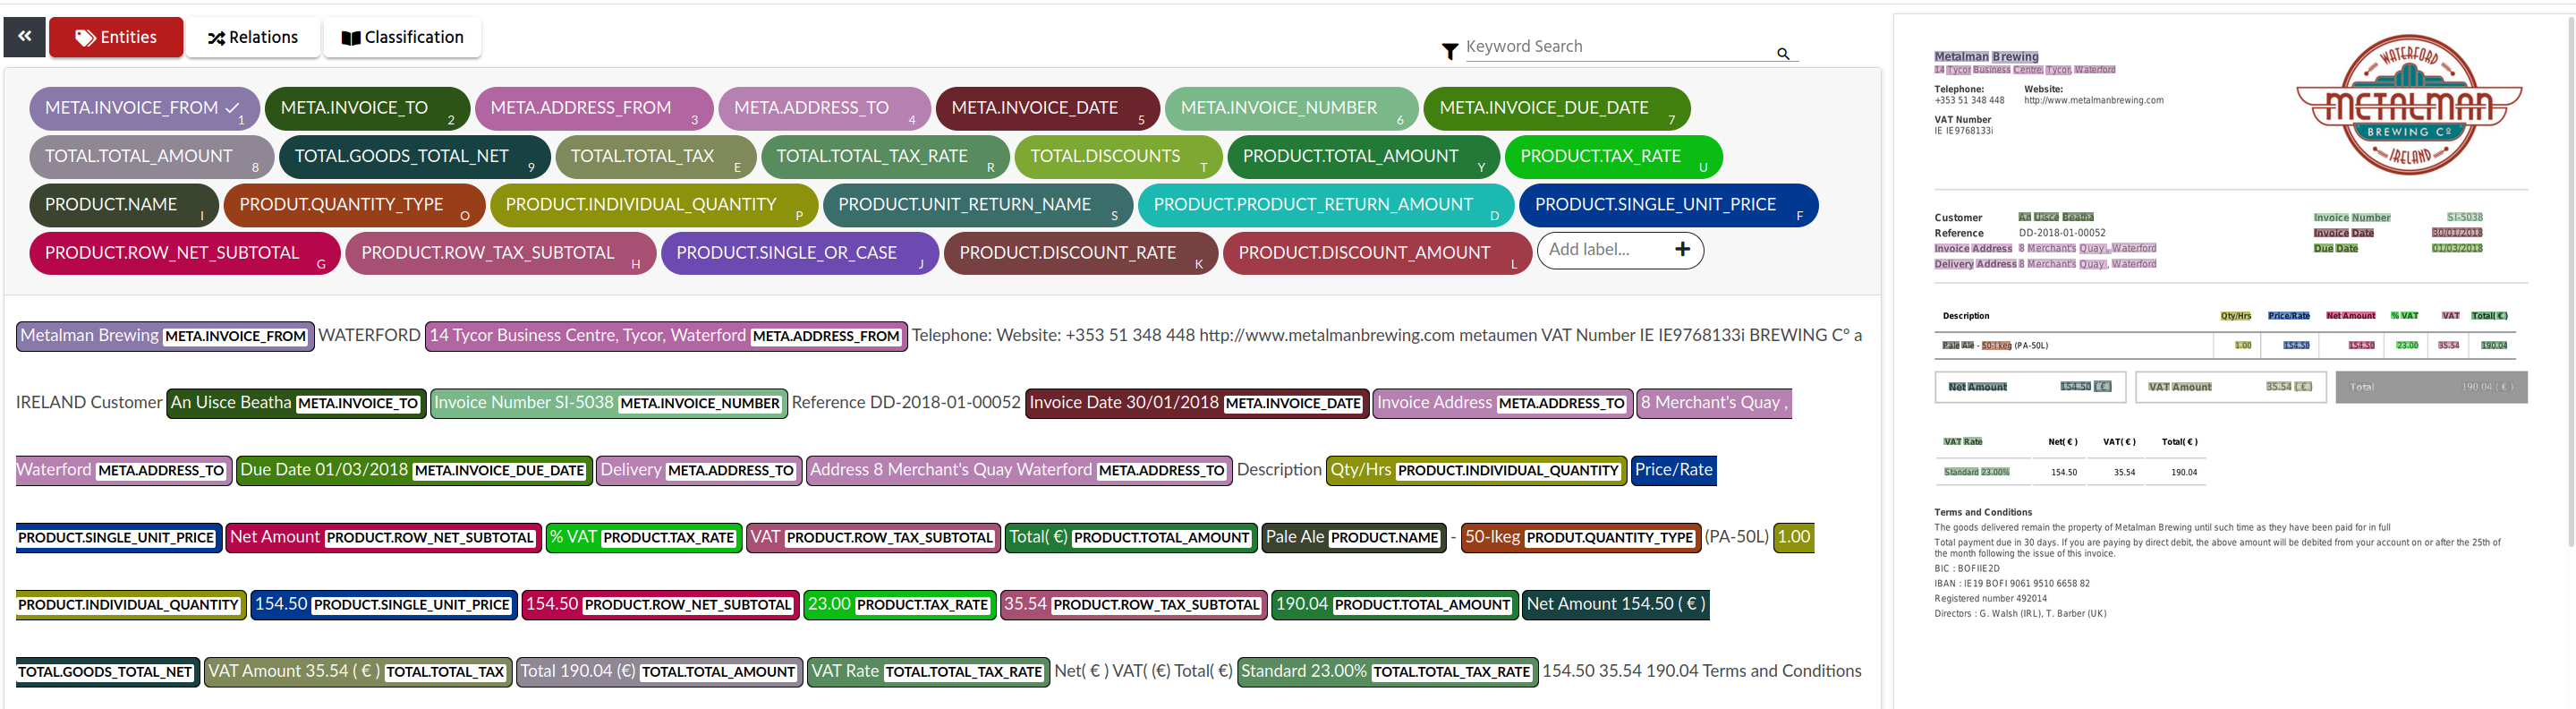
\includegraphics[width=1\textwidth]{figures/ubiai_annotate.png}
		      \caption{Annotating the dataset using UBIAI Annotation Tool}
		      \label{fig:training_annotations}
	      \end{figure}
	      Even with this enhanced workflow, the annotation process was still very time-consuming. In total 86 documents
	      were annotated. Whilst this isn't an ideal amount, the larger the training set the better the model can
	      learn, research showed that from approx. 50 documents LayoutLMv2 was able to return decent results.\\
	      This finding was corroborated by Walid.
	\item \textbf{Exporting the Data}: the data is exported from the UBIAI software in an optimized format for the transformers
	      based architecture model. There appears to be a wide range of different options for data. With UBIAI supporting these methods:
	      \begin{figure}[H]
		      \centering
		      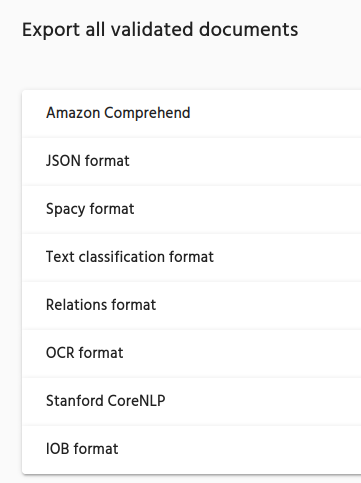
\includegraphics[width=0.35\textwidth]{figures/ubiai_export_options.png}
		      \caption{UBIAI Export Options}
		      \label{fig:ubiai_export_options}
	      \end{figure}
	      If the data is not exported in the correct format it can take a large amount of time to transform the data into a
	      suitable format for the model.\\
	      The documents are exported along with some metadata files which contain the labels and the bounding boxes for each
	      document.
\end{enumerate}
% \begin{wrapfigure}{r}{0.35\textwidth}
% 	\centering
% 	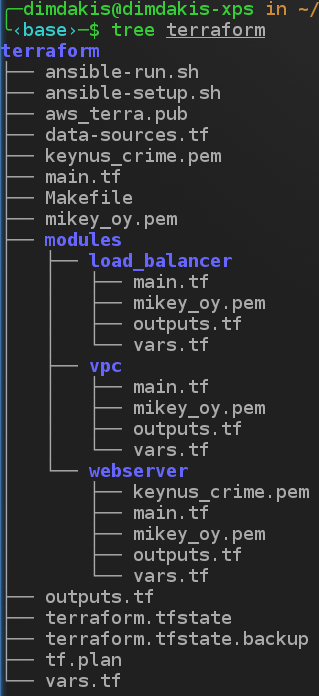
\includegraphics[width=0.3\textwidth]{figures/terra_dir_struct.png}
% 	\caption{The Terraform project structure}
% 	\label{fig:terra_project_structure}
% \end{wrapfigure}
\section{Training the Model}
With the data in the correct format and the labels created, the next step is to train the model. The training script
is written in Python, and it utilizes a number of libraries. Including the following:
\begin{itemize}
	\item \textbf{PyTorch}: the main framework for the model.
	\item \textbf{torchvision}: the library for image processing.
	\item \textbf{transformers}: the library for the model and processor.
	\item \textbf{Detectron2}: the library for object detection.
	\item
\end{itemize}
There is still quite a bit of processing to do before the model can be trained. The data is manipulated to arrive at a
pandas dataframe of as per \Cref{fig:training_dataframe}:
\begin{figure}[H]
	\centering
	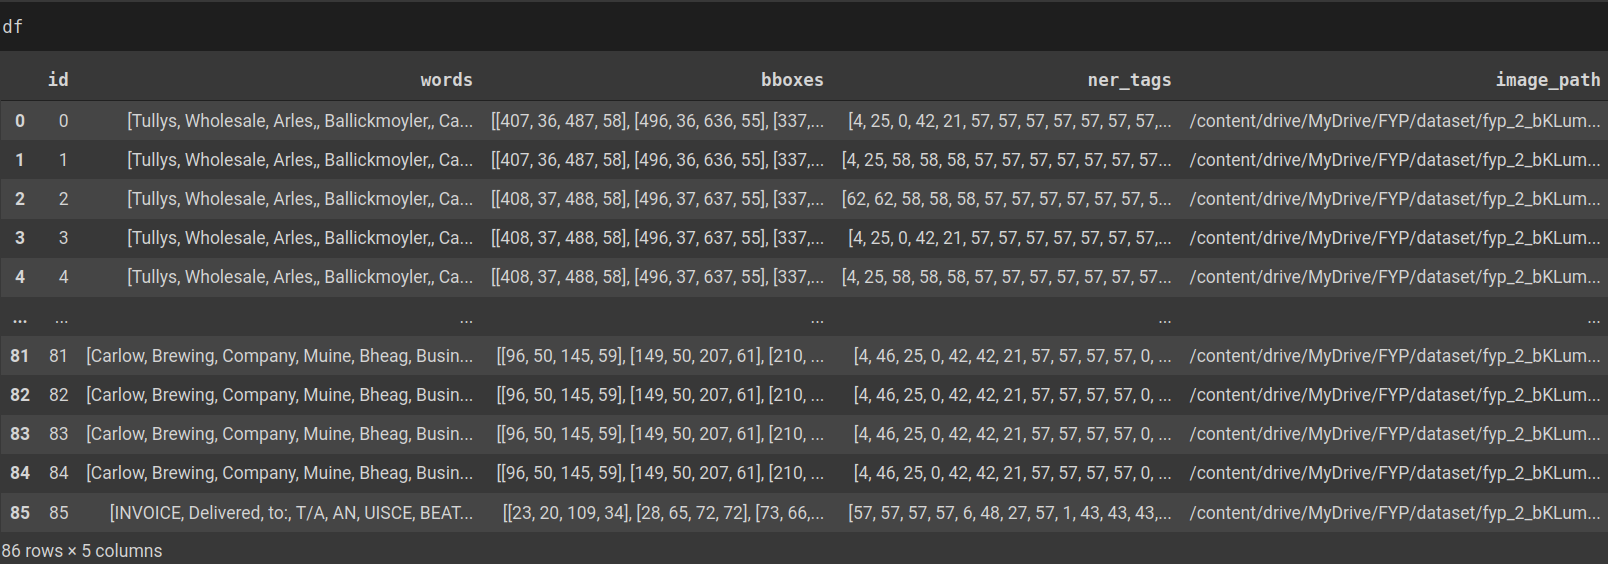
\includegraphics[width=1\textwidth]{figures/training_dataframe.png}
	\caption{Training Dataframe}
	\label{fig:training_dataframe}
\end{figure}
It is important to note that each row in the dataframe represents a single document (invoice). For this training run,
there were 86 documents annotated, therefore, there are 86 rows in the dataframe. The columns are as follows:
\begin{itemize}
	\item \textbf{id}: the id of the document, incrementing from 0 to 85.
	\item \textbf{words}: this is a list of every OCR'd word in the document.
	\item \textbf{bboxes}: this is a list of bounding boxes (the four coordinates of the box) for each word in the document.
	      the bounding boxes need to be normalized. This is done by dividing the bounding box coordinates by the width and height:
	      \begin{lstlisting}[language=python, label={lst:bbox_normalization}, caption={Bounding Box Normalization}]
	def normalize_bbox(bbox, width, height):
    return [
        int(1000 * (bbox[0] / width)),
        int(1000 * (bbox[1] / height)),
        int(1000 * (bbox[2] / width)),
        int(1000 * (bbox[3] / height)),
    ]
	\end{lstlisting}
	\item \textbf{ner\_tags}: the Named Entity Relation (NER) tags for each word in the document. These are the labels
	      that were applied to the words. There is some minor processing done, to get to this stage. The labels are
	      encoded as integers and any word that doesn't have a label is assigned the label `0'.
	      \bigbreak
	      There are now more labels than were present initially. This is due to the giving the model some extra information,
	      where each prefix letter is has a meaning. This meaning corresponds to the token position of the token in an entity.\\
	      The token prefixes are as follows:
	      \begin{itemize}
		      \item \textbf{B} - Beginning of a new entity.
		      \item \textbf{I} - Inside an entity. For example, the `State' token is a part of an entity like `Empire State Building`.
		            this means the ner\_tag would have a a prefix of \code{I\_}~\autocite{TokenClassification}
		      \item \textbf{S} - This denotes a single token entity.
		      \item \textbf{E} - The token is the end of an entity.
		      \item \textbf{O} - Doesn't correspond to any entity.
	      \end{itemize}
	      The amount of elements in in the word, bboxes and ner\_tags columns should be equal.
		
	\item \textbf{image\_path}: the path to the image file.
\end{itemize}
\bigbreak
The LayoutLMv2 model in this project is used in \emph{TokenClassification} mode. \\
\#\#\ explain Tokenisation and the WordPiece Algo used by LayoutLMv2 ? \#\#\
\subsection{Data for Model Training}
\begin{itemize}
	\item As we prep the model needs to be trained. For the training of the model the dataset needs to be prepared.
	      \begin{itemize}
		      \item annotation and correct export of data.
	      \end{itemize}
	\item The model needs to be saved
	\item The
\end{itemize}